\chapter{Laravel Blade Template}

Blade เป็น PHP Templating Engine ที่ถูกพัฒนาโดยผู้พัฒนา Laravel Framework 
โดย Blade Templates จะถูก compile เป็น code ภาษา PHP 
และถูกเก็บเป็น Cached ไว้ที่ directory \mintinline{bash}{app/storage/framework/views} จนกว่าจะมีการเปลี่ยนแปลงโค้ด Blade ใหม่

ไฟล์ Blade จะมีนามสกุล \mintinline{bash}{.blade.php} และต้องสร้างไฟล์ Blade 
ไว้ใน directory \mintinline{bash}{resources/views} และการแสดงผลของไฟล์ Blade 
จะถือเป็นส่วน View ของ MVC (Model-View-Controller Architectural Pattern)

\section{Template Inheritance}

สิ่งหนึ่งที่ต้องจัดการเสมอในการออกแบบหน้าเว็บ คือ ทุกหน้าควรมีรูปแบบในทำนองเดียวกัน (Consistency) 
และคุณสมบัติหนึ่งที่ Blade Templates ช่วยในเรื่องนี้ คือ Template Inheritance 
โดยแบ่งออกเป็น 2 ส่วน คือ Master Layout และ Child View

Master Layout เป็นการวางโครงสร้างของหน้าเว็บ เพื่อให้ทุกหน้ามีรูปแบบโครงสร้างเดียวกัน เพื่อคงคุณลักษณะ Consistency ของการแสดงผลของเว็บไซต์
โดยแต่ละหน้าจะมีการแสดงผลใน Child View ที่แตกต่างกัน ซึ่งจะเลือก Master Layout มาใช้ในการแสดงผลสำหรับแต่ละ Child View ด้วย

\newpage

\subsection{การเขียน Master Layout}

สร้างไฟล์ \mintinline{bash}{resources/views/layouts/main.blade.php}

\begin{code}{html}{resources/views/layouts/main.blade.php}{}
    <!DOCTYPE html>
    <html lang="en">
    <head>
        <meta charset="UTF-8">
        <meta name="viewport" 
            content="width=device-width, initial-scale=1.0">
        <meta http-equiv="X-UA-Compatible" content="ie=edge">
        <title>My App</title>
        <link rel="stylesheet" href="{{ url('css/app.css') }}">
    </head>
    <body>
        @include('layouts.menu')
        
        <div class="container mt-2">
            @yield('content')
        </div>
    
        <script src="{{ url('js/app.js') }}"></script>
    
    </body>
    </html>
\end{code}

Directive \mintinline{php}{@include} ใช้แสดงเนื้อหาจากไฟล์ที่กำหนด 
โดยระบุในรูปแบบ Dot Notation เช่น \mintinline{php}{layouts.menu} หมายถึงไฟล์ \mintinline{bash}{resources/views/layouts/menu.blade.php} ซึ่งจะนำมาแทรกที่จุดดังกล่าว

Directive \mintinline{php}{@yield} ใช้แสดงเนื้อหาที่กำหนดใน directive \mintinline{php}{@section} ชื่อเดียวกัน ที่จะเขียนใน Child View

\newpage

สร้างไฟล์ \mintinline{bash}{resources/views/layouts/menu.blade.php} เพื่อนำไป include ใน layouts.main

\begin{code}{html}{resources/views/layouts/menu.blade.php}{}
    <nav class="navbar is-primary" 
         role="navigation" aria-label="main navigation">
        <div class="navbar-brand">
            <a class="navbar-item" href="/">
                My App
            </a>

            <a role="button" data-target="navMenu" class="navbar-burger" 
               aria-label="menu" aria-expanded="false">
                <span aria-hidden="true"></span>
                <span aria-hidden="true"></span>
                <span aria-hidden="true"></span>
            </a>
        </div>
        <div class="navbar-menu" id="navMenu">
            <a class="navbar-item">
                Home
            </a>
        </div>
    </nav>


\end{code}

\subsection{การเขียน Child View}

สร้างไฟล์ \mintinline{bash}{resources/views/about.blade.php}

\begin{code}{html}{resources/views/about.blade.php}{}
    @extends('layouts.main')

    @section('content')
        <h1 class="is-size-1">About Us</h1>
        <p>My App is Demo App</p>
    @endsection

\end{code}

ในไฟล์ Child View จะต้องระบุไฟล์ Layout ที่ต้องการใช้งานเป็นโครงสร้างหลักของหน้า 
ไว้ใน \mintinline{php}{@extends} Directive ซึ่งจะต้องระบุเป็นรูปแบบ Dot Notation 
เช่น \mintinline{php}{layouts.main} หมายถึงไฟล์ \mintinline{bash}{resources/views/layouts/main.blade.php}

\subsection{การใช้งาน CSS/JS Framework}

Laravel 8 ไม่ได้กำหนด CSS Framework เริ่มต้นให้ เหมือนที่ Laravel 7 กำหนด Bootstrap เป็น CSS Framework ไว้เป็นค่าเริ่มต้นให้
ในหัวข้อนี้จะแนะนำวิธีการใช้งานเบื้องต้น

1. เปิดการใช้งาน node package manager
\begin{cli}{}
    npm install
\end{cli}

2. ติดตั้ง Bulma หากต้องการ CSS Framework อื่น ให้ค้นหาวิธีการติดตั้ง ซึ่งจะมีรูปแบบคล้ายกัน
\begin{cli}{}
    npm install bulma
\end{cli}

3. สร้างไฟล์ \mintinline{bash}{resources/css/sass/app.scss}

\begin{code}{css}{resources/css/sass/app.scss}{}
    @charset "utf-8";

    @import '~bulma/bulma.sass';
\end{code}

4. แก้ไขไฟล์ \mintinline{bash}{resources/js/app.js}

\begin{code}{javascript}{resources/js/app.js}{}
    require('./bootstrap');

    document.addEventListener('DOMContentLoaded', () => {

        // Get all "navbar-burger" elements
        const $navbarBurgers = Array.prototype.slice
                .call(document.querySelectorAll('.navbar-burger'), 0);

        // Check if there are any navbar burgers
        if ($navbarBurgers.length > 0) {
            // Add a click event on each of them
            $navbarBurgers.forEach( el => {
                el.addEventListener('click', () => {

                    // Get the target from the "data-target" attribute
                    const target = el.dataset.target;
                    const $target = document.getElementById(target);

                    // Toggle the "is-active" class on both the "navbar-burger" and the "navbar-menu"
                    el.classList.toggle('is-active');
                    $target.classList.toggle('is-active');
                });
            });
        }
    });
\end{code}

5. แก้ไขไฟล์ \mintinline{bash}{webpack.mix.js}

\begin{code}{javascript}{webpack.mix.js}{}
const mix = require('laravel-mix');

mix.js('resources/js/app.js', 'public/js')
    .sass('resources/css/sass/app.scss', 'public/css', [
        //
    ]);
\end{code}

6. จากนั้นใช้คำสั่ง npm run dev เพื่อ preprocess 
\begin{cli}{}
    npm run dev
\end{cli}

\begin{out}{}
DONE  Compiled successfully in 4306ms

       Asset     Size   Chunks             Chunk Names
/css/app.css  232 KiB  /js/app  [emitted]  /js/app
  /js/app.js  595 KiB  /js/app  [emitted]  /js/app
\end{out}

จะได้ไฟล์ \mintinline{bash}{public/css/app.css} และ \mintinline{bash}{public/js/app.js}
ซึ่งถูกนำไปใช้ใน \mintinline{php}{layouts.main}

\newpage

กำหนด route เพื่อแสดงหน้า about
\begin{code}{php}{routes/web.php}{}
    <?php
    // ...
    Route::get('/about', function () {
        return view('about');
    });
\end{code}


ทดสอบเรียกหน้า localhost:8000/about จะเห็นว่าได้ Layout ตามที่กำหนดไว้ใน \mintinline{php}{layouts.main}

\begin{figure}[h!]
    \centering
    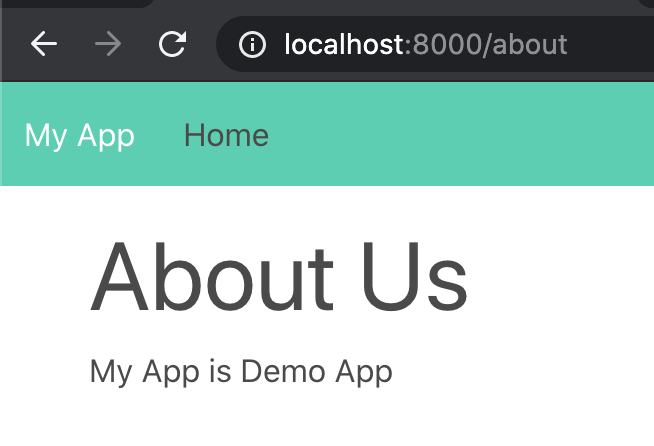
\includegraphics[width=0.6\textwidth]{images/ch4/01.png}
    \caption{หน้าเว็บที่เรียกไปยัง route /about}
\end{figure}

\newpage

\section{การแสดงข้อมูลใน Blade Template}

สามารถส่งข้อมูล Associative Array เป็น parameter ที่ 2 ในฟังก์ชัน \mintinline{php}{view()} เพื่อนำไปแสดงผลใน Blade Template เช่น

\begin{code}{php}{routes/web.php}{}
    <?php
    // ...
    Route::get('/about', function () {
        return view('about', [
            'name' => 'Your Name',
            'info' => [
                'address' => 'Bangkok, <b>Thailand</b>',
                'email' => 'contact@example.com'
            ] 
        ]);
    });
\end{code}

โดย key ของ Associative Array จะเป็นชื่อตัวแปรใน Blade Template จากตัวอย่าง ทำให้ในไฟล์ Blade Template 
มีตัวแปร \mintinline{php}{$name} ที่มีค่า \mintinline{php}{'Your Name'} และมีตัวแปร \mintinline{php}{$info} ที่มีค่า 
\mintinline{php}{['address' => 'Bangkok, <b>Thailand</b>', 'email' => 'contact@example.com']}

การแสดงข้อมูลใน Blade Templates จะใช้ double curly braces (\mintinline{php}{{{  }}}) statement เช่น 

\begin{code}{php}{resources/views/about.blade.php}{}
    @extends('layouts.main')

    @section('content')
        <h1 class="is-size-1">About Us</h1>
        <p>My App is Demo App</p>

        <div class="card">
            <div class="card-content">
                <div class="media">
                    <div class="media-content">
                        <p class="title is-4">{{ $name }}</p>
                        <p class="subtitle is-6">{{ $info['email'] }}</p>
                    </div>
                </div>
                <div class="content">
                    {{ $info['address'] }}
                </div>
            </div>
        </div>
    @endsection
\end{code}

\begin{figure}[h!]
    \centering
    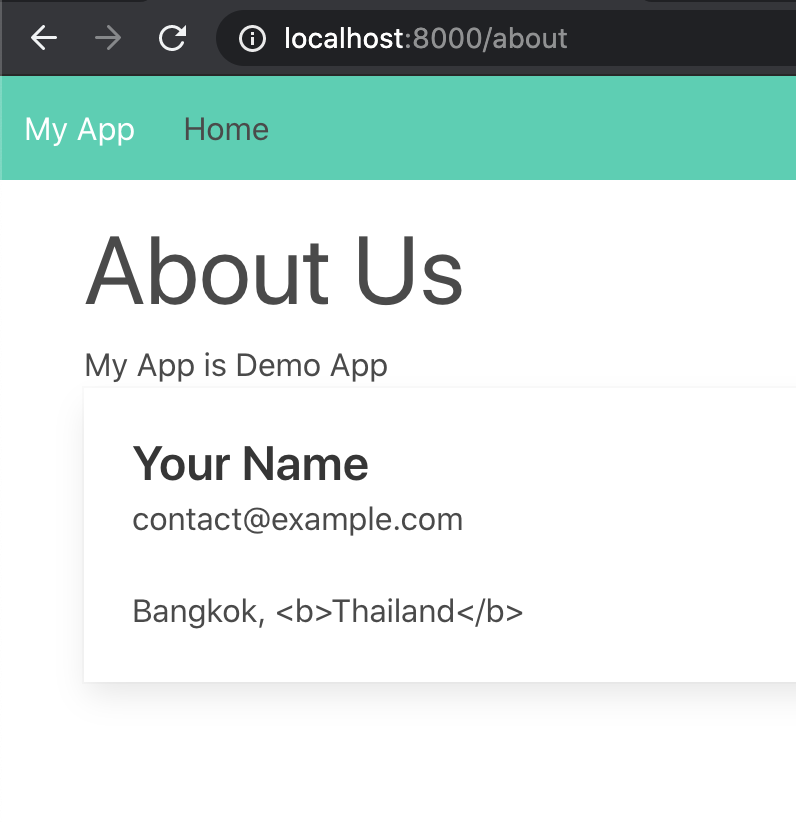
\includegraphics[width=0.6\textwidth]{images/ch4/02.png}
    \caption{หน้าเว็บที่เรียกไปยัง localhost:8000/about และมีการส่งข้อมูลไปแสดง}
\end{figure}

ซึ่ง \mintinline{php}{{{ }}} statement จะนำค่าในตัวแปรไปผ่านฟังก์ชัน \mintinline{php}{htmlspecialchars()} ของ PHP เพื่อป้องกัน XSS Attack 
หรือเรียกว่าเป็นการแสดงข้อมูลแบบ escaped (ตัวอย่าง Tag <b> ไม่ถูกประมวลผลเป็น HTML จึงไม่แสดง Thailand เป็นตัวหนา และแสดง <b> ให้ปรากฏบน browser)
\newpage
หากต้องการแสดงข้อมูลแบบ unescaped data ให้ใช้ \mintinline{php}{{!! !!}} statement แทน เช่น 

\begin{code}{php}{ตัวอย่าง Blade Syntax แสดงข้อมูลแบบ unescaped}{}
    {!! $info['address'] !!}
\end{code}

\begin{figure}[h!]
    \centering
    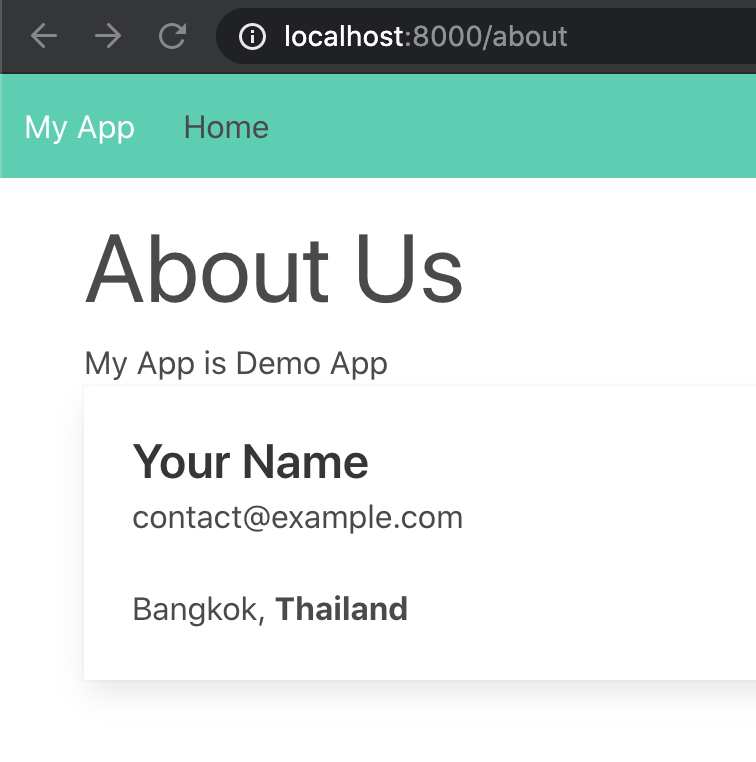
\includegraphics[width=0.6\textwidth]{images/ch4/03.png}
    \caption{ตัวอย่างการแสดงข้อมูลแบบ unescaped}
\end{figure}
\newpage
หากไม่ต้องการให้ประมวลผล Blade Syntax ให้ใส่ @ นำหน้า เช่น \mintinline{php}{@{{ name }}} ซึ่งในบาง JavaScript Framework จะใช้ \mintinline{javascript}{{{ }}} ในการแสดงข้อมูลเช่นกัน

\begin{code}{php}{ตัวอย่าง Blade Syntax ที่ไม่ต้องการแสดงผล Blade Syntax}{}
    @{{ $name }}
\end{code}

\begin{figure}[h!]
    \centering
    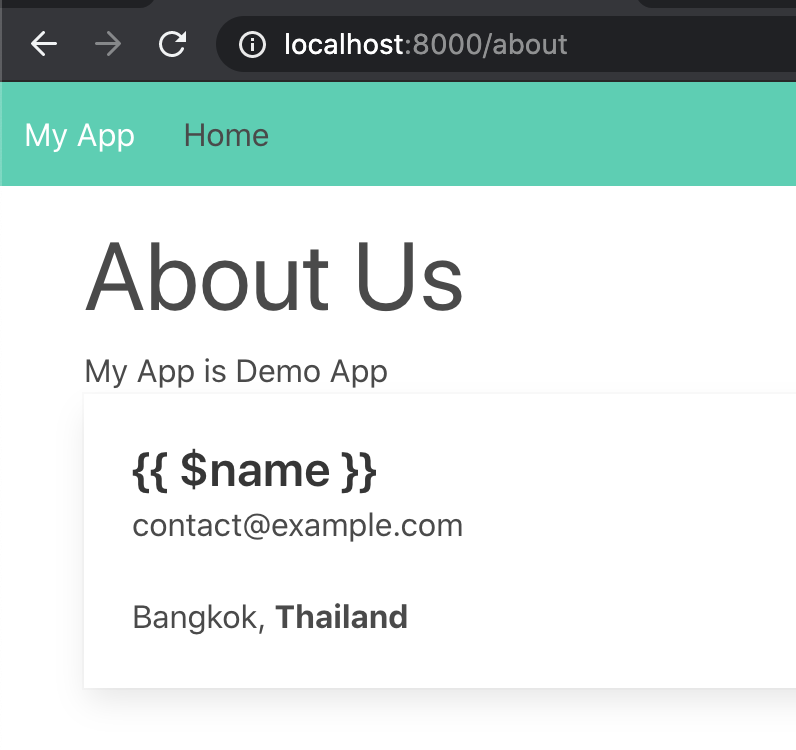
\includegraphics[width=0.6\textwidth]{images/ch4/04.png}
    \caption{ตัวอย่างการแสดงข้อมูลที่ไม่ต้องการประมวลผล Blade Syntax}
\end{figure}

\newpage

\section{Blade Control Structure}
Blade Template สามารถใช้ if statement โดยใช้ \mintinline{php}{@if}, \mintinline{php}{@elseif}, \mintinline{php}{@else} และ \mintinline{php}{@endif} directives ซึ่งเมื่อถูกคอมไพล์ จะเปลี่ยนเป็น if statement ของภาษา PHP

\begin{code}{php}{Blade Control Structure: if}{}
    @if (count($records) === 1)
        I have one record!
    @elseif (count($records) > 1)
        I have multiple records!
    @else
        I don't have any records!
    @endif
\end{code}

หรือการใช้งาน Loop

\begin{code}{php}{Blade Control Structure: for}{}
    @for ($i = 0; $i < 5; $i++)
        <p>The current value is {{ $i }}</p>
    @endfor

    @foreach ($users as $user)
        <p>This is user {{ $user->id }}</p>
    @endforeach

\end{code}

ศึกษา Blade Templates และ Blade Syntax เพิ่มเติมได้ที่ \\
\href{https://laravel.com/docs/8.x/blade}{https://laravel.com/docs/8.x/blade}